% ============================================================
%  ADI Model Zoo — Beamer Slide Deck
%  Compile: pdflatex ADI_ModelZoo_Slides.tex
% ============================================================
\documentclass[aspectratio=169,10pt]{beamer}

% ── Packages ────────────────────────────────────────────────
\usepackage[T1]{fontenc}
\usepackage[utf8]{inputenc}
\usepackage{lmodern}
\usepackage{microtype}
\usepackage{booktabs}
\usepackage{array}
\usepackage{multirow}
\usepackage{colortbl}
\usepackage{xcolor}
\usepackage{tikz}
\usepackage{pgfplots}
\pgfplotsset{compat=1.18}
\usepackage{listings}
\usepackage{fontawesome5}
\usepackage{calc}
\usetikzlibrary{arrows.meta,shapes.geometric,positioning,fit,backgrounds,shadows,decorations.pathreplacing}

% ── ADI Brand Colors ─────────────────────────────────────────
\definecolor{ADIBlue}{RGB}{0,102,204}
\definecolor{ADITeal}{RGB}{0,155,119}
\definecolor{ADIDark}{RGB}{20,20,40}
\definecolor{ADIGray}{RGB}{100,100,100}
\definecolor{ADILightGray}{RGB}{240,242,245}
\definecolor{ADIAmber}{RGB}{255,163,0}
\definecolor{ADIRed}{RGB}{210,35,42}
\definecolor{ADIGreen}{RGB}{0,180,80}

% ── Theme Setup ──────────────────────────────────────────────
\usetheme{Madrid}
\usecolortheme[named=ADIBlue]{structure}

\setbeamercolor{palette primary}{bg=ADIBlue,fg=white}
\setbeamercolor{palette secondary}{bg=ADIDark,fg=white}
\setbeamercolor{palette tertiary}{bg=ADIBlue!80!ADIDark,fg=white}
\setbeamercolor{palette quaternary}{bg=ADIDark,fg=white}
\setbeamercolor{titlelike}{parent=palette primary}
\setbeamercolor{frametitle}{bg=ADIBlue,fg=white}
\setbeamercolor{block title}{bg=ADIBlue,fg=white}
\setbeamercolor{block body}{bg=ADIBlue!8}
\setbeamercolor{alerted text}{fg=ADITeal}
\setbeamercolor{block title alerted}{bg=ADITeal,fg=white}
\setbeamercolor{block body alerted}{bg=ADITeal!8}
\setbeamercolor{item}{fg=ADIBlue}
\setbeamercolor{subitem}{fg=ADITeal}
\setbeamercolor{footline}{bg=ADIDark,fg=white}
\setbeamercolor{headline}{bg=ADIBlue}
\setbeamertemplate{navigation symbols}{}
\setbeamertemplate{itemize item}{\textcolor{ADIBlue}{\textbullet}}
\setbeamertemplate{itemize subitem}{\textcolor{ADITeal}{$\triangleright$}}
\setbeamerfont{frametitle}{series=\bfseries,size=\normalsize}

% ── Code Listing Style ───────────────────────────────────────
\lstset{
  basicstyle=\ttfamily\scriptsize,
  keywordstyle=\color{ADIBlue}\bfseries,
  commentstyle=\color{ADIGray},
  stringstyle=\color{ADITeal},
  backgroundcolor=\color{ADILightGray},
  frame=single,
  framerule=0.4pt,
  rulecolor=\color{ADIBlue!40},
  breaklines=true,
  showstringspaces=false,
  tabsize=2,
}

% ── Helpers ──────────────────────────────────────────────────
\newcommand{\adi}[1]{\textcolor{ADIBlue}{\textbf{#1}}}
\newcommand{\teal}[1]{\textcolor{ADITeal}{\textbf{#1}}}
\newcommand{\highlight}[1]{\colorbox{ADIBlue!12}{\strut #1}}
\newcommand{\chipbadge}[1]{\tikz[baseline=-0.5ex]\node[draw=ADIBlue,fill=ADIBlue!10,
  rounded corners=2pt,inner sep=2pt,font=\scriptsize\bfseries\color{ADIBlue}]{#1};}

% ── Title Info ───────────────────────────────────────────────
\title[ADI Model Zoo]{ADI Model Zoo: Embedded AI for Edge \& Sensor Applications}
\subtitle{Analog Devices Inc.\ Pre-trained Model Collection\\
  for MAX78002 / MAX32690 / ADSP-SC835}
\author{Analog Devices, Inc.}
\date{2026}

% ============================================================
\begin{document}
% ============================================================

% ── TITLE SLIDE ─────────────────────────────────────────────
\begin{frame}[plain]
  \begin{tikzpicture}[remember picture,overlay]
    \fill[ADIDark] (current page.south west) rectangle (current page.north east);
    \fill[ADIBlue] (current page.south west) rectangle ([yshift=3.2cm]current page.south east);
    \fill[ADITeal!70!ADIBlue] ([yshift=3.2cm]current page.south west)
      rectangle ([yshift=3.6cm]current page.south east);
    \node[anchor=south west,inner sep=0] at ([xshift=1cm,yshift=3.7cm]current page.south west) {
      \begin{minipage}{0.85\paperwidth}
        {\color{white}\fontsize{18}{22}\selectfont\bfseries ADI Model Zoo}\\[4pt]
        {\color{ADITeal!80!white}\fontsize{12}{15}\selectfont Embedded AI for Edge \& Sensor Applications}\\[6pt]
        {\color{white!70}\fontsize{9}{11}\selectfont
          Analog Devices Inc.\ Pre-trained Model Collection for\\
          \textbf{MAX78002} / \textbf{MAX32690} / \textbf{ADSP-SC835}}
      \end{minipage}
    };
    \node[anchor=south east,inner sep=1cm] at (current page.south east) {
      {\color{ADIBlue!40}\fontsize{8}{10}\selectfont github.com/analogdevicesinc/adi-model-zoo}
    };
    % stat boxes
    \foreach \val/\lbl/\xoff in {%
      {15+}/{Models}/0,%
      {3}/{Domains}/3.5,%
      {3}/{Platforms}/7.0}{
      \node[draw=ADITeal,fill=ADIDark!80,rounded corners=4pt,
            inner sep=6pt,text=white,anchor=south,
            font=\scriptsize] at ([xshift=\xoff cm+1.5cm,yshift=0.3cm]current page.south west){
        {\fontsize{16}{18}\selectfont\bfseries\color{ADITeal}\val}\\[2pt]\lbl
      };
    }
  \end{tikzpicture}
\end{frame}

% ── OVERVIEW 1: What Is ADI Model Zoo ────────────────────────
\begin{frame}{ADI Model Zoo — Overview}
  \begin{columns}[T]
    \column{0.55\textwidth}
    \begin{block}{What It Is}
      A curated collection of \alert{pretrained ML models} targeting\\
      Analog Devices \textbf{ultra-low-power} embedded hardware.
      \vspace{4pt}
      \begin{itemize}
        \item \alert{15+} models across 3 application domains
        \item \alert{3} target hardware platforms
        \item Models stored \textbf{directly in the repo}\\
              (no link-file indirection)
        \item Self-contained, runnable with a single command
      \end{itemize}
    \end{block}
    \vspace{4pt}
    \begin{alertblock}{Key Differentiator}
      TinyML-first: every model is designed for\\
      \textbf{microwatt-to-milliwatt} deployment on MCU + CNN silicon.
    \end{alertblock}

    \column{0.42\textwidth}
    \begin{block}{Three Domains}
      \begin{tabular}{@{}ll@{}}
        \chipbadge{VISION}  & 7 models \\[4pt]
        \chipbadge{AUDIO}   & 5 models \\[4pt]
        \chipbadge{SENSOR}  & 3 models \\
      \end{tabular}
    \end{block}
    \vspace{4pt}
    \begin{block}{Repository}
      {\small\ttfamily github.com/analogdevicesinc/adi-model-zoo}\\[4pt]
      {\small\textbf{model\_index.json} — central registry\\
      \textbf{models.schema.json} — JSON Schema validation}
    \end{block}
  \end{columns}
\end{frame}

% ── OVERVIEW 2: Per-Model Structure ─────────────────────────
\begin{frame}{Self-Contained Model Structure}
  \begin{columns}[T]
    \column{0.48\textwidth}
    \begin{block}{Every Model Directory Contains}
      \begin{tikzpicture}[
        dir/.style={draw=ADIBlue,fill=ADIBlue!8,rounded corners=2pt,
                    font=\scriptsize\ttfamily,inner sep=3pt,minimum width=3.5cm},
        file/.style={draw=ADIGray!50,fill=white,rounded corners=2pt,
                     font=\scriptsize\ttfamily,inner sep=3pt,minimum width=3.5cm},
        every node/.style={anchor=west},
        level distance=5mm,
        sibling distance=4mm
      ]
        \node[dir] {\faFolder\ <model>/}
          child { node[dir] {\faFolder\ data/}
            child { node[file] {\faFile\ input/} }
            child { node[file] {\faFile\ model/ (.pth.tar/.tflite)} }
            child { node[file] {\faFile\ output/ (reference)} }
          }
          child[yshift=-22pt] { node[dir] {\faFolder\ data\_processing/} }
          child[yshift=-34pt] { node[file] {\faFile\ definition.yaml} }
          child[yshift=-46pt] { node[file] {\faFile\ example.py} }
          child[yshift=-58pt] { node[file] {\faFile\ README.md} }
          child[yshift=-70pt] { node[file] {\faFile\ requirements.txt} };
      \end{tikzpicture}
    \end{block}

    \column{0.48\textwidth}
    \begin{block}{definition.yaml (Schema-Validated)}
      \begin{lstlisting}[language=yaml,basicstyle=\ttfamily\tiny]
version: "1.0"
schema_type: "edge_ai_model"
model:
  name: "DS-CNN Small"
  formats:
    - format: "TFLite"
      model_files:
        - name: "ds_cnn_s_int8.tflite"
          precision: "INT8"
          size_mb: 0.097
  metadata:
    license:
      model: {name: "Apache-2.0"}
  inputs:
    - name: "input"
      shape: [1, 490]
      dtype: "float32"
  outputs:
    - name: "identity"
      shape: [1, 12]
      dtype: "float32"
      \end{lstlisting}
    \end{block}
    \vspace{4pt}
    \begin{alertblock}{Run Any Model}
      {\small\ttfamily\$ python example.py data/input/input.jpg}
    \end{alertblock}
  \end{columns}
\end{frame}

% ── HARDWARE 1: Platform Table ───────────────────────────────
\begin{frame}{Target Hardware Platforms}
  \renewcommand{\arraystretch}{1.35}
  \begin{tabular}{@{}>{\bfseries\color{ADIBlue}}l
                  >{\small}l >{\small}l >{\small}l >{\small}l@{}}
    \toprule
    \textcolor{black}{Device} & Family & Core & Memory & Key Capability \\
    \midrule
    \rowcolor{ADIBlue!8}
    MAX78002
      & DARWIN CNN
      & CM4F + CNN accel
      & 384\,KB SRAM, 2\,MB flash
      & 74-layer CNN, \alert{$<$6\,mW}, 1024-ch \\
    MAX32690
      & DARWIN MCU
      & Cortex-M4F
      & 3\,MB flash, 1\,MB SRAM
      & BLE 5.2, USB, ultra-low-power \\
    \rowcolor{ADIBlue!8}
    ADSP-SC835
      & Blackfin+ DSP
      & DSP + Arm
      & On-chip SRAM + DDR
      & HiFi4 DSP, audio/voice \\
    \bottomrule
  \end{tabular}

  \vspace{0.6cm}
  \begin{columns}[T]
    \column{0.3\textwidth}
    \begin{block}{\chipbadge{MAX78002} CNN Accelerator}
      {\small
      \begin{itemize}
        \item Hardware CNN engine: up to 74 layers
        \item Max 1024 channels per layer
        \item Integer-only weights (INT8)
        \item Active power \alert{$<$6\,mW}
      \end{itemize}}
    \end{block}
    \column{0.3\textwidth}
    \begin{block}{\chipbadge{MAX32690} MCU}
      {\small
      \begin{itemize}
        \item Cortex-M4F @ 120\,MHz
        \item TFLite Micro inference
        \item BLE 5.2 + USB
        \item 3\,MB flash for models
      \end{itemize}}
    \end{block}
    \column{0.3\textwidth}
    \begin{block}{\chipbadge{ADSP-SC835} DSP}
      {\small
      \begin{itemize}
        \item HiFi4 DSP core + Arm
        \item Real-time audio/DSP
        \item PyTorch FP32 capable
        \item Blackfin+ architecture
      \end{itemize}}
    \end{block}
  \end{columns}
\end{frame}

% ── HARDWARE 2: Performance Chart ───────────────────────────
\begin{frame}{Platform Compute Performance}
  \begin{columns}[T]
    \column{0.55\textwidth}
    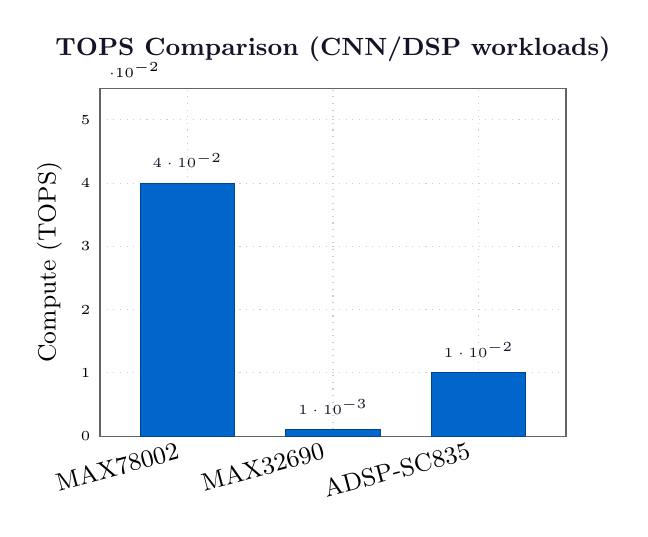
\begin{tikzpicture}
      \begin{axis}[
        ybar,
        width=7.5cm, height=6cm,
        bar width=1.2cm,
        symbolic x coords={MAX78002,MAX32690,ADSP-SC835},
        xtick=data,
        x tick label style={font=\small,rotate=15,anchor=east},
        ylabel={Compute (TOPS)},
        ylabel style={font=\small},
        ymin=0, ymax=0.055,
        ytick={0,0.01,0.02,0.03,0.04,0.05},
        yticklabel style={font=\tiny},
        grid=major,
        grid style={dotted,gray!40},
        tick style={draw=none},
        axis line style={ADIGray},
        enlarge x limits=0.3,
        nodes near coords,
        nodes near coords style={font=\tiny,color=ADIDark},
        every node near coord/.append style={yshift=2pt},
        title={TOPS Comparison (CNN/DSP workloads)},
        title style={font=\small\bfseries,color=ADIDark},
      ]
        \addplot[fill=ADIBlue,draw=ADIBlue!70!black] coordinates {
          (MAX78002, 0.040)
          (MAX32690, 0.001)
          (ADSP-SC835, 0.010)
        };
      \end{axis}
    \end{tikzpicture}

    \column{0.42\textwidth}
    \vspace{0.3cm}
    \begin{block}{Power Profile}
      \renewcommand{\arraystretch}{1.2}
      \begin{tabular}{@{}l r@{}}
        \toprule
        Device & Active Power \\
        \midrule
        MAX78002 CNN & \alert{$<$6\,mW} \\
        MAX78002 MCU & $\sim$15\,mW \\
        MAX32690 & $\sim$8\,mW \\
        ADSP-SC835 & $\sim$500\,mW \\
        \bottomrule
      \end{tabular}
    \end{block}
    \vspace{4pt}
    \begin{alertblock}{TinyML Focus}
      MAX78002 delivers \alert{$\sim$0.04\,TOPS} at under \alert{6\,mW} — ideal for battery-powered and energy-harvesting edge nodes.
    \end{alertblock}
    \vspace{4pt}
    \begin{block}{Use Case Fit}
      {\small
      \begin{itemize}
        \item CNN vision/audio: \textbf{MAX78002}
        \item MCU inference + BLE: \textbf{MAX32690}
        \item DSP audio/signal: \textbf{ADSP-SC835}
      \end{itemize}}
    \end{block}
  \end{columns}
\end{frame}

% ── HARDWARE 3: Eval Boards & Dev Flow ──────────────────────
\begin{frame}{Evaluation Boards \& Development Flow}
  \begin{columns}[T]
    \column{0.45\textwidth}
    \begin{block}{Evaluation Kits}
      \renewcommand{\arraystretch}{1.3}
      \begin{tabular}{@{}ll@{}}
        \toprule
        SoC & Eval Board \\
        \midrule
        MAX78002 & MAX78002EVKIT \\
        MAX32690 & EvKit\_V1 \\
        ADSP-SC835 & ADSPSC835-EV-SOM \\
        \bottomrule
      \end{tabular}
      \vspace{6pt}
      \begin{itemize}\small
        \item Camera + mic headers
        \item UART debug console
        \item USB power + JTAG
      \end{itemize}
    \end{block}

    \column{0.52\textwidth}
    \begin{block}{Development Flow}
      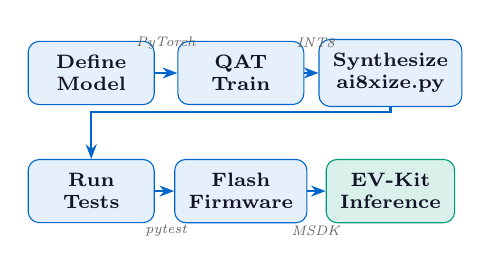
\begin{tikzpicture}[
        box/.style={draw=ADIBlue,fill=ADIBlue!10,rounded corners=4pt,
                    font=\scriptsize\bfseries,inner sep=5pt,
                    minimum width=1.6cm,minimum height=0.7cm,
                    text=ADIDark,align=center},
        arr/.style={-{Stealth[scale=0.8]},thick,color=ADIBlue},
        note/.style={font=\tiny\itshape,color=ADIGray,align=center}
      ]
        \node[box] (A) at (0,0) {Define\\Model};
        \node[box] (B) at (1.9,0) {QAT\\Train};
        \node[box] (C) at (3.8,0) {Synthesize\\ai8xize.py};
        \node[box] (D) at (0,-1.5) {Run\\Tests};
        \node[box] (E) at (1.9,-1.5) {Flash\\Firmware};
        \node[box,fill=ADITeal!15,draw=ADITeal] (F) at (3.8,-1.5) {EV-Kit\\Inference};
        \draw[arr] (A)--(B);
        \draw[arr] (B)--(C);
        \draw[arr] (C)--++(0,-0.5)--++(-3.8,0)--(D);
        \draw[arr] (D)--(E);
        \draw[arr] (E)--(F);
        \node[note] at (0.95,0.38) {PyTorch};
        \node[note] at (2.85,0.38) {INT8};
        \node[note] at (0.95,-2.0) {pytest};
        \node[note] at (2.85,-2.0) {MSDK};
      \end{tikzpicture}
    \end{block}
  \end{columns}
  \vspace{0.3cm}
  \begin{block}{MSDK — MAX Software Development Kit}
    {\small Complete SDK for MAX78000/MAX78002/MAX32690: BSP, drivers, peripheral examples, TFLite Micro integration, and pre-built EV-Kit demo firmware.}
  \end{block}
\end{frame}

% ── MODEL DOMAINS OVERVIEW ───────────────────────────────────
\begin{frame}{Model Domains at a Glance}
  \begin{columns}[T]
    \column{0.32\textwidth}
    \begin{block}{\textcolor{ADIBlue}{\faEye\ Vision} — 7 Models}
      \vspace{4pt}
      \begin{tabular}{@{}ll@{}}
        \textbf{Task} & \textbf{\#} \\
        \midrule
        Image Classification & 3 \\
        Image Segmentation & 1 \\
        Object Detection & 2 \\
        Visual Wake Word & 1 \\
      \end{tabular}
      \vspace{4pt}

      \chipbadge{MAX78002} \chipbadge{MAX32690}\\[4pt]
      Formats: AI8X, TFLite INT8
    \end{block}

    \column{0.32\textwidth}
    \begin{block}{\textcolor{ADITeal}{\faMicrophone\ Audio} — 5 Models}
      \vspace{4pt}
      \begin{tabular}{@{}ll@{}}
        \textbf{Task} & \textbf{\#} \\
        \midrule
        Audio Denoising & 2 \\
        Genre Identification & 1 \\
        Keyword Spotting & 2 \\
      \end{tabular}
      \vspace{4pt}

      \chipbadge{MAX78002} \chipbadge{MAX32690} \chipbadge{SC835}\\[4pt]
      Formats: AI8X, TFLite, PyTorch
    \end{block}

    \column{0.32\textwidth}
    \begin{block}{\textcolor{ADIAmber}{\faIndustry\ Sensor} — 3 Models}
      \vspace{4pt}
      \begin{tabular}{@{}ll@{}}
        \textbf{Task} & \textbf{\#} \\
        \midrule
        Motor Fault Detection & 1 \\
        Anomaly Detection & 2 \\
      \end{tabular}
      \vspace{4pt}

      \chipbadge{MAX78002} \chipbadge{MAX32690}\\[4pt]
      Formats: AI8X INT8, TFLite
    \end{block}
  \end{columns}

  \vspace{0.4cm}
  
\begin{tikzpicture}
    \fill[ADIBlue] (0,0) rectangle (0.32\textwidth-2pt,4pt);
    \fill[ADITeal] (0.34\textwidth,0) rectangle (0.66\textwidth,4pt);
    \fill[ADIAmber] (0.68\textwidth,0) rectangle (\textwidth-2pt,4pt);
  \end{tikzpicture}
\end{frame}

% ── FORMATS 1: Three Formats ─────────────────────────────────
\begin{frame}{Model Formats}
  \begin{columns}[T]
    \column{0.32\textwidth}
    \begin{block}{\adi{AI8X} (ADI Proprietary)}
      {\small
      \begin{itemize}
        \item PyTorch layers constrained to MAX78000/78002 hardware limits
        \item Weights: \texttt{.pth.tar} \\Network: \texttt{.py}
        \item INT8 QAT (Quantization-Aware Training)
        \item Synthesized via \texttt{ai8xize.py}
        \item Produces per-layer CNN hardware config
      \end{itemize}}
      \vspace{4pt}
      \chipbadge{MAX78002} primary
    \end{block}

    \column{0.32\textwidth}
    \begin{block}{\teal{TFLite}}
      {\small
      \begin{itemize}
        \item FP32, INT16, and INT8 variants
        \item TFLite Micro runtime on MAX32690
        \item Multi-precision per model:\\
          \texttt{int8} / \texttt{int16} / \texttt{float32}
        \item Compilation flags:\\
          \texttt{-O0} (accuracy) / \texttt{-O2} (speed)
        \item ADSP-SC835: FP32 TFLite
      \end{itemize}}
      \vspace{4pt}
      \chipbadge{MAX32690} \chipbadge{SC835}
    \end{block}

    \column{0.32\textwidth}
    \begin{block}{\textbf{PyTorch (.pt)}}
      {\small
      \begin{itemize}
        \item FP32 only
        \item ADSP-SC835 only\\(has sufficient compute)
        \item Used by:\\
          \textit{GenreNet Conv2D} (15.3\,MB)
        \item Standard PyTorch \texttt{torch.load()} inference
        \item No hardware compilation needed
      \end{itemize}}
      \vspace{4pt}
      \chipbadge{ADSP-SC835} only
    \end{block}
  \end{columns}

  \vspace{0.4cm}
  \begin{alertblock}{Format Selection Guide}
    {\small \textbf{Battery-powered vision/audio} → AI8X (MAX78002)\quad
    \textbf{MCU + wireless} → TFLite (MAX32690)\quad
    \textbf{DSP audio pipeline} → PyTorch (ADSP-SC835)}
  \end{alertblock}
\end{frame}

% ── FORMATS 2: AI8X Deep Dive ───────────────────────────────
\begin{frame}{AI8X Format — Deep Dive}
  \begin{columns}[T]
    \column{0.52\textwidth}
    \begin{block}{Hardware Constraints (MAX78002)}
      {\small
      \begin{itemize}
        \item Max \alert{74 sequential CNN layers}
        \item Max \alert{1024 channels} per layer
        \item Weight precision: \textbf{INT8 only}
        \item No arbitrary activations (ReLU, abs, max)
        \item Limited pooling options per layer
      \end{itemize}}
    \end{block}
    \vspace{4pt}
    \begin{block}{Channel Folding}
      {\small When an image is too large for the channel limit,\\
      \texttt{ai8x.fold(fold\_ratio)} \textit{interlaces} spatial pixels into channels:}
      \vspace{4pt}
      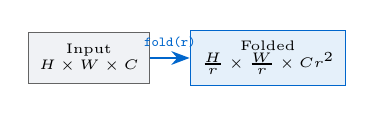
\begin{tikzpicture}
        \node[draw=ADIGray,fill=ADILightGray,inner sep=4pt,font=\tiny,align=center] (A)
          {Input\\$H \times W \times C$};
        \node[draw=ADIBlue,fill=ADIBlue!10,inner sep=4pt,font=\tiny,align=center,right=0.5cm of A] (B)
          {Folded\\$\frac{H}{r} \times \frac{W}{r} \times Cr^2$};
        \draw[-{Stealth},ADIBlue,thick] (A)--(B) node[midway,above,font=\tiny]{\texttt{fold(r)}};
      \end{tikzpicture}
      {\small\par Enables larger receptive fields within 1024-channel limit.}
    \end{block}

    \column{0.45\textwidth}
    \begin{block}{AI8X Synthesis Pipeline}
      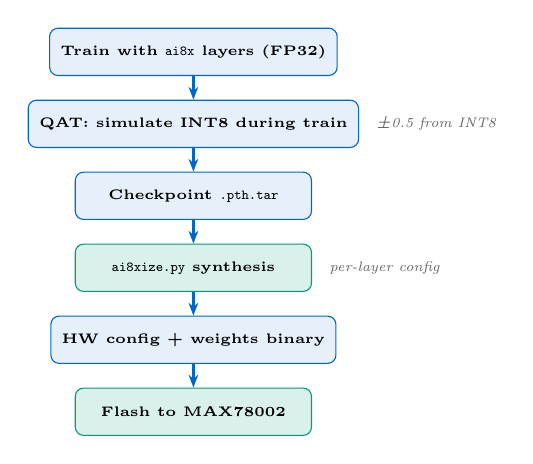
\begin{tikzpicture}[
        box/.style={draw=ADIBlue,fill=ADIBlue!10,rounded corners=3pt,
                    font=\tiny\bfseries,inner sep=4pt,minimum width=3cm,
                    minimum height=0.6cm,align=center},
        gbox/.style={box,fill=ADITeal!15,draw=ADITeal},
        arr/.style={-{Stealth[scale=0.7]},ADIBlue,thick},
        lbl/.style={font=\tiny\itshape,color=ADIGray}
      ]
        \node[box] (T) {Train with \texttt{ai8x} layers (FP32)};
        \node[box,below=0.3cm of T] (Q) {QAT: simulate INT8 during train};
        \node[box,below=0.3cm of Q] (C) {Checkpoint \texttt{.pth.tar}};
        \node[gbox,below=0.3cm of C] (S) {\texttt{ai8xize.py} synthesis};
        \node[box,below=0.3cm of S] (H) {HW config + weights binary};
        \node[gbox,below=0.3cm of H] (F) {Flash to MAX78002};
        \draw[arr] (T)--(Q);
        \draw[arr] (Q)--(C);
        \draw[arr] (C)--(S);
        \draw[arr] (S)--(H);
        \draw[arr] (H)--(F);
        \node[lbl,right=0.1cm of Q] {±0.5 from INT8};
        \node[lbl,right=0.1cm of S] {per-layer config};
      \end{tikzpicture}
    \end{block}
    \vspace{4pt}
    \begin{alertblock}{Normalization}
      {\small Input normalized to \alert{[$-$128, 127]}:\\
      $x' = \text{round}((x - 0.5) \times 256)$\\
      clamped to INT8 range before CNN engine.}
    \end{alertblock}
  \end{columns}
\end{frame}

% ── VISION 1: Classification ─────────────────────────────────
\begin{frame}{Vision Models — Image Classification}
  \begin{columns}[T]
    \column{0.55\textwidth}
    \renewcommand{\arraystretch}{1.2}
    \begin{tabular}{@{}>{\small\bfseries}l >{\small}l >{\small}c >{\small}c >{\small}r@{}}
      \toprule
      Model & Dataset & Input & Top-1 & Size \\
      \midrule
      \rowcolor{ADIBlue!8}
      EfficientNetV2 & ImageNet & 112$\times$112 & \alert{0.6197} & 19.9\,MB \\
      MobileNetV2 0.75$\times$ & CIFAR-100 & 32$\times$32 & \alert{0.6471} & 10.5\,MB \\
      \rowcolor{ADIBlue!8}
      MobileNetV2 0.5$\times$ & CIFAR-100 & 32$\times$32 & $\sim$0.62 & 5.12\,MB \\
      SimpleNet & CIFAR-100 & 32$\times$32 & \alert{0.6030} & 8.40\,MB \\
      \bottomrule
    \end{tabular}
    \vspace{4pt}
    {\small All models: \chipbadge{MAX78002} AI8X INT8 via QAT}

    \vspace{6pt}
    \begin{block}{Model Highlights}
      {\small
      \begin{itemize}
        \item \textbf{EfficientNetV2}: Compound-scaled, 1000-class ImageNet
        \item \textbf{MobileNetV2}: Inverted residuals, depthwise-separable, 100-class CIFAR-100; two width multipliers (0.75×, 0.5×)
        \item \textbf{SimpleNet}: Sequential conv blocks, lightweight, 100-class
      \end{itemize}}
    \end{block}

    \column{0.42\textwidth}
    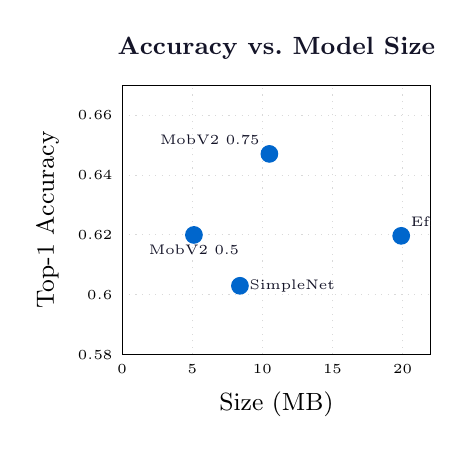
\begin{tikzpicture}
      \begin{axis}[
        width=5.5cm, height=5cm,
        xlabel={Size (MB)}, ylabel={Top-1 Accuracy},
        xlabel style={font=\small},
        ylabel style={font=\small},
        xmin=0, xmax=22,
        ymin=0.58, ymax=0.67,
        grid=major, grid style={dotted,gray!30},
        tick style={draw=none},
        ticklabel style={font=\tiny},
        title={Accuracy vs.\ Model Size},
        title style={font=\small\bfseries,color=ADIDark},
      ]
        \addplot[only marks,mark=*,mark size=3pt,color=ADIBlue] coordinates {
          (19.9, 0.6197)
          (10.5, 0.6471)
          (5.12, 0.62)
          (8.40, 0.6030)
        };
        \node[font=\tiny,above right,color=ADIDark] at (axis cs:19.9,0.6197) {EffNetV2};
        \node[font=\tiny,above left,color=ADIDark]  at (axis cs:10.5,0.6471) {MobV2 0.75};
        \node[font=\tiny,below,color=ADIDark]       at (axis cs:5.12,0.62)   {MobV2 0.5};
        \node[font=\tiny,right,color=ADIDark]       at (axis cs:8.40,0.6030) {SimpleNet};
      \end{axis}
    \end{tikzpicture}
  \end{columns}
\end{frame}

% ── VISION 2: Segmentation + Detection ──────────────────────
\begin{frame}{Vision Models — Segmentation \& Detection}
  \begin{columns}[T]
    \column{0.48\textwidth}
    \begin{block}{\faShapes\ Image Segmentation}
      \textbf{U-Net}\\[4pt]
      \renewcommand{\arraystretch}{1.2}
      \begin{tabular}{@{}ll@{}}
        Dataset   & AISegment (person/background) \\
        Input     & 48$\times$48$\times$48 (folded 3-ch) \\
        Accuracy  & \alert{0.9845} \\
        Format    & AI8X INT8 \\
        Size      & 3.23\,MB \\
        Target    & \chipbadge{MAX78002} \\
      \end{tabular}
      \vspace{4pt}
      {\small Encoder–decoder with skip connections.\\
      Pixel-wise binary segmentation.}
    \end{block}

    \column{0.48\textwidth}
    \begin{block}{\faSearch\ Object Detection}
      \textbf{FeaturePyramidNet}\\[2pt]
      {\small Multi-scale FPN, Pascal VOC 21-class}
      \begin{itemize}\small
        \item Input: 256$\times$320, mAP: \alert{0.505}
        \item Output: 10\,200 anchors (loc + cls)
        \item AI8X INT8, 25.16\,MB, \chipbadge{MAX78002}
      \end{itemize}
      \vspace{4pt}
      \textbf{TinierSSD (QR Code)}\\[2pt]
      {\small Single-shot detector with keypoints}
      \begin{itemize}\small
        \item Input: 120$\times$160, mAP: \alert{0.900}
        \item 4 corner keypoints per QR code
        \item AI8X INT8, 4.46\,MB, \chipbadge{MAX78002}
      \end{itemize}
    \end{block}
  \end{columns}

  \vspace{0.3cm}
  \begin{alertblock}{NMS Post-Processing (FPN)}
    {\small\ttfamily from data\_processing.utils import object\_detection\_utils as od\\
    boxes, labels, scores = od.detect\_objects(locs, scores, num\_classes=21, ...)}
  \end{alertblock}
\end{frame}

% ── VISION 3: Visual Wake Word ───────────────────────────────
\begin{frame}{Vision Models — Visual Wake Word}
  \begin{columns}[T]
    \column{0.5\textwidth}
    \begin{block}{MicroNet VWW2 INT8}
      \renewcommand{\arraystretch}{1.3}
      \begin{tabular}{@{}ll@{}}
        \toprule
        Property & Value \\
        \midrule
        Task      & Person / No-person detection \\
        Dataset   & Visual Wake Words (COCO-based) \\
        Input     & 50$\times$50$\times$1 (greyscale) \\
        Output    & 2-class softmax \\
        Accuracy  & \alert{0.768} \\
        Format    & TFLite \textbf{INT8} \\
        Size      & \alert{267\,KB} \\
        Target    & \chipbadge{MAX32690} \\
        Runtime   & TFLite Micro (Cortex-M4F) \\
        \bottomrule
      \end{tabular}
    \end{block}

    \column{0.47\textwidth}
    \begin{block}{Architecture}
      MicroNet — neural architecture designed for\\
      TinyML on commodity MCUs:\\[4pt]
      {\small
      \begin{itemize}
        \item Grouped + depthwise-separable convolutions
        \item $\sim$500K parameters
        \item INT8 quantization, 267\,KB fits in MAX32690 flash
        \item Inference: $\sim$10–20\,ms on CM4F @ 120\,MHz
      \end{itemize}}
    \end{block}
    \vspace{4pt}
    \begin{alertblock}{Always-On Use Case}
      {\small Runs continuously at \textbf{$<$1\,mW}, waking a more\\
      powerful pipeline only when a person is detected.}
    \end{alertblock}
    \vspace{4pt}
    \begin{block}{Preprocessing}
      {\small Greyscale convert → resize to 50$\times$50 →\\
      normalize INT8 → TFLite Micro invoke}
    \end{block}
  \end{columns}
\end{frame}

% ── AUDIO 1: Denoising ──────────────────────────────────────
\begin{frame}{Audio Models — Denoising}
  \begin{columns}[T]
    \column{0.48\textwidth}
    \begin{block}{DTLN — Dual-Signal Transformation LSTM}
      \renewcommand{\arraystretch}{1.2}
      \begin{tabular}{@{}ll@{}}
        Metric    & PESQ \alert{2.950} \\
        Format    & TFLite FP32 (×2 models) \\
        Sizes     & 1.39\,MB + 2.39\,MB \\
        Params    & $<$1\,M \\
        Sample rate & 16\,kHz \\
        Frame     & 32\,ms \\
      \end{tabular}
      \vspace{6pt}
      {\small Two-stage: STFT-domain mask + learned analysis/synthesis basis. Stateful — 4 state tensors persist between frames.}\\[4pt]
      {\small\textit{Authors: Westhausen \& Meyer (Interspeech 2020)}}
    \end{block}

    \column{0.48\textwidth}
    \begin{block}{RNNoise}
      \renewcommand{\arraystretch}{1.2}
      \begin{tabular}{@{}ll@{}}
        Metric    & PESQ \alert{2.945} \\
        Format    & TFLite \textbf{INT8} \\
        Size      & \alert{107\,KB} \\
        Target    & \chipbadge{MAX32690} \\
        Frame     & 10\,ms \\
        Features  & 42 Bark-band features \\
      \end{tabular}
      \vspace{6pt}
      {\small GRU-based: VAD GRU (24) → Noise GRU (48) → Denoise GRU (96). Outputs spectral mask (22 bands) + VAD confidence.}\\[4pt]
      {\small\textit{Author: Jean-Marc Valin (Mozilla)}}
    \end{block}
  \end{columns}

  \vspace{0.4cm}
  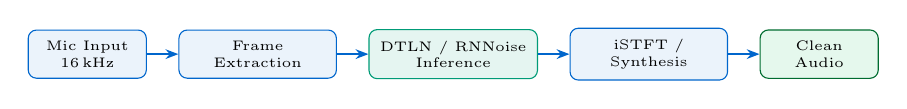
\begin{tikzpicture}[
    box/.style={draw=ADIBlue,fill=ADIBlue!8,rounded corners=3pt,font=\tiny,
                inner sep=4pt,minimum height=0.6cm,align=center},
    arr/.style={-{Stealth[scale=0.7]},ADIBlue,thick}
  ]
    \node[box,minimum width=1.5cm] (A) {Mic Input\\16\,kHz};
    \node[box,minimum width=2cm,right=0.4cm of A] (B) {Frame\\Extraction};
    \node[box,minimum width=2cm,right=0.4cm of B,fill=ADITeal!10,draw=ADITeal] (C) {DTLN / RNNoise\\Inference};
    \node[box,minimum width=2cm,right=0.4cm of C] (D) {iSTFT /\\Synthesis};
    \node[box,minimum width=1.5cm,right=0.4cm of D,fill=ADIGreen!10,draw=ADIGreen!60!black] (E) {Clean\\Audio};
    \draw[arr] (A)--(B); \draw[arr] (B)--(C); \draw[arr] (C)--(D); \draw[arr] (D)--(E);
  \end{tikzpicture}
\end{frame}

% ── AUDIO 2: KWS + Genre ────────────────────────────────────
\begin{frame}{Audio Models — Keyword Spotting \& Genre ID}
  \begin{columns}[T]
    \column{0.32\textwidth}
    \begin{block}{\adi{DS-CNN Small}}
      {\small
      \begin{itemize}
        \item Accuracy: \alert{94.52\%}
        \item Dataset: Speech Commands V2
        \item Classes: \textbf{12 keywords}
        \item Format: TFLite INT8/INT16/FP32
        \item Size: \alert{97\,KB} (INT8)
        \item Input: 1$\times$490 MFCC features
        \item Output: 1$\times$12 softmax
      \end{itemize}}
      \vspace{2pt}
      \chipbadge{MAX32690} \chipbadge{ADSP-SC835}\\[2pt]
      {\tiny ARM Research / Stanford}
    \end{block}

    \column{0.32\textwidth}
    \begin{block}{\adi{Conv1D AudioNet}}
      {\small
      \begin{itemize}
        \item Accuracy: \alert{86.34\%}
        \item Dataset: Speech Commands V2
        \item Classes: \textbf{20 keywords}
        \item Format: AI8X INT8
        \item Size: 1.785\,MB
        \item Input: 128$\times$128 spectrogram
      \end{itemize}}
      \vspace{4pt}
      \chipbadge{MAX78002}\\[2pt]
      {\tiny Cornell University (Zhang et al.)}
    \end{block}

    \column{0.32\textwidth}
    \begin{block}{\adi{GenreNet Conv2D}}
      {\small
      \begin{itemize}
        \item Accuracy: \alert{84.50\%}
        \item Dataset: GTZAN
        \item Classes: \textbf{10 genres}
        \item Format: PyTorch FP32
        \item Size: 15.3\,MB
        \item Input: 1$\times$1$\times$128$\times$128 Mel spectrogram
      \end{itemize}}
      \vspace{4pt}
      \chipbadge{ADSP-SC835}\\[2pt]
      {\tiny Vellore Institute of Tech.}
    \end{block}
  \end{columns}

  \vspace{0.4cm}
  \begin{block}{Audio KWS Preprocessing}
    {\small 16\,kHz audio → 1-second window → MFCC / log-mel features → model input tensor → argmax class prediction}
  \end{block}
\end{frame}

% ── SENSOR 1: Motor Fault ───────────────────────────────────
\begin{frame}{Sensor Models — Motor Fault Detection}
  \begin{columns}[T]
    \column{0.52\textwidth}
    \begin{block}{Convolutional Autoencoder}
      \renewcommand{\arraystretch}{1.3}
      \begin{tabular}{@{}ll@{}}
        \toprule
        Property & Value \\
        \midrule
        Task      & Motor fault / degradation \\
        Dataset   & ADI Motor Data (Limerick) \\
        Input     & 256$\times$3 (3-axis vibration) \\
        Output    & 256$\times$3 (reconstructed) \\
        Metric    & MSE: \alert{0.02205} \\
        Format    & AI8X \textbf{INT8} \\
        Size      & 1.59\,MB \\
        Target    & \chipbadge{MAX78002} \\
        Fault     & High reconstruction MSE \\
        \bottomrule
      \end{tabular}
    \end{block}

    \column{0.45\textwidth}
    \begin{block}{Fault Detection Principle}
      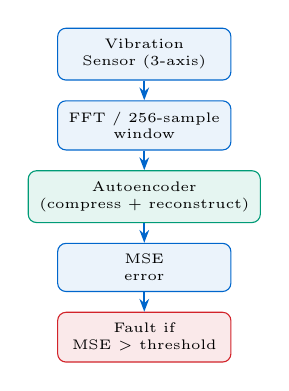
\begin{tikzpicture}[
        box/.style={draw=ADIBlue,fill=ADIBlue!8,rounded corners=3pt,
                    font=\tiny,inner sep=4pt,align=center,minimum width=2.2cm},
        arr/.style={-{Stealth[scale=0.7]},ADIBlue,thick}
      ]
        \node[box] (S) {Vibration\\Sensor (3-axis)};
        \node[box,below=0.25cm of S] (F) {FFT / 256-sample\\window};
        \node[box,below=0.25cm of F,fill=ADITeal!10,draw=ADITeal] (AE) {Autoencoder\\(compress + reconstruct)};
        \node[box,below=0.25cm of AE] (E) {MSE\\error};
        \node[box,below=0.25cm of E,fill=ADIRed!10,draw=ADIRed] (D) {Fault if\\MSE $>$ threshold};
        \draw[arr] (S)--(F); \draw[arr] (F)--(AE);
        \draw[arr] (AE)--(E); \draw[arr] (E)--(D);
      \end{tikzpicture}
    \end{block}
    \vspace{4pt}
    \begin{alertblock}{Principle}
      {\small Trained only on \textbf{normal} motor signals. High reconstruction error on anomalous/faulty signal.}
    \end{alertblock}
  \end{columns}
\end{frame}

% ── SENSOR 2: Anomaly Detection ─────────────────────────────
\begin{frame}{Sensor Models — Anomaly Detection}
  \begin{columns}[T]
    \column{0.48\textwidth}
    \begin{block}{Autoencoder ×4 (MIMII)}
      {\small Per-machine-type variants:}
      \vspace{4pt}
      \begin{tabular}{@{}llr@{}}
        \toprule
        Variant & Machine & Size \\
        \midrule
        \texttt{model\_fan\_quant} & Fan & 287\,KB \\
        \texttt{model\_pump\_quant} & Pump & 287\,KB \\
        \texttt{model\_slider\_quant} & Slider & 287\,KB \\
        \texttt{model\_valve\_quant} & Valve & 287\,KB \\
        \bottomrule
      \end{tabular}
      \vspace{4pt}
      {\small AUC: \alert{0.516}, pAUC: 0.523\\
      Dataset: MIMII (industrial machine sounds)\\
      Input: 196$\times$640 spectrogram\\
      Format: TFLite FP32, \chipbadge{MAX32690}}
    \end{block}

    \column{0.48\textwidth}
    \begin{block}{MicroNet AD Small}
      \renewcommand{\arraystretch}{1.2}
      \begin{tabular}{@{}ll@{}}
        Architecture & Lightweight CNN \\
        Approach     & Self-supervised machine-ID \\
        Dataset      & DCASE 2020 / MIMII rail \\
        Input        & 32$\times$32$\times$1 log-mel \\
        Output       & 4-class machine ID \\
        Format       & TFLite \textbf{INT8} \\
        Size         & \alert{240\,KB} \\
        Target       & \chipbadge{MAX32690} \\
      \end{tabular}
      \vspace{4pt}
      {\small\textit{Anomaly = low confidence in known machine-ID class. No anomaly labels needed for training.}}
    \end{block}
  \end{columns}

  \vspace{0.2cm}
  \begin{alertblock}{Self-Supervised Anomaly Detection}
    {\small Train as a \textbf{normal-class classifier} (machine type / operating condition). At inference, low predicted class confidence → anomaly alert. No anomaly labels required during training.}
  \end{alertblock}
\end{frame}

% ── QUANTIZATION 1: AI8X QAT ────────────────────────────────
\begin{frame}{Quantization \& Deployment — AI8X QAT}
  \begin{columns}[T]
    \column{0.52\textwidth}
    \begin{block}{QAT Flow}
      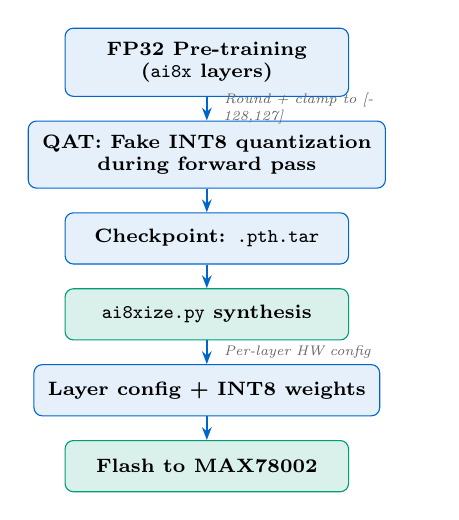
\begin{tikzpicture}[
        box/.style={draw=ADIBlue,fill=ADIBlue!10,rounded corners=3pt,
                    font=\scriptsize\bfseries,inner sep=5pt,
                    minimum width=3.6cm,minimum height=0.65cm,align=center},
        gbox/.style={box,fill=ADITeal!15,draw=ADITeal},
        arr/.style={-{Stealth[scale=0.7]},ADIBlue,thick},
        note/.style={font=\tiny\itshape,color=ADIGray,text width=2.5cm}
      ]
        \node[box] (A) {FP32 Pre-training\\(\texttt{ai8x} layers)};
        \node[box,below=0.3cm of A] (B) {QAT: Fake INT8 quantization\\during forward pass};
        \node[box,below=0.3cm of B] (C) {Checkpoint: \texttt{.pth.tar}};
        \node[gbox,below=0.3cm of C] (D) {\texttt{ai8xize.py} synthesis};
        \node[box,below=0.3cm of D] (E) {Layer config + INT8 weights};
        \node[gbox,below=0.3cm of E] (F) {Flash to MAX78002};
        \draw[arr] (A)--(B) node[note,right=0.1cm,midway]{Round + clamp to [-128,127]};
        \draw[arr] (B)--(C);
        \draw[arr] (C)--(D);
        \draw[arr] (D)--(E) node[note,right=0.1cm,midway]{Per-layer HW config};
        \draw[arr] (E)--(F);
      \end{tikzpicture}
    \end{block}

    \column{0.45\textwidth}
    \begin{block}{INT8 Specification}
      {\small
      \begin{itemize}
        \item Range: \alert{[$-$128, 127]}
        \item Per-layer weight quantization
        \item Channel folding: $r^2\times$ channel expansion, $r\times$ spatial reduction
        \item Normalization: $x' = \text{round}((x - 0.5) \cdot 256)$
        \item Bias: INT8, per-channel
      \end{itemize}}
    \end{block}
    \vspace{4pt}
    \begin{block}{Accuracy Retention}
      {\small QAT simulates INT8 error during training, so the model's learned weights compensate. Typical INT8 accuracy drop $<$1--2\%.}
    \end{block}
    \vspace{4pt}
    \begin{alertblock}{Key Insight}
      {\small Unlike post-training quantization, QAT models are \textbf{trained} for INT8 deployment — accuracy drop is minimized at the training stage.}
    \end{alertblock}
  \end{columns}
\end{frame}

% ── QUANTIZATION 2: TFLite Multi-Precision ──────────────────
\begin{frame}{Quantization \& Deployment — TFLite}
  \begin{columns}[T]
    \column{0.5\textwidth}
    \begin{block}{Multi-Precision TFLite (DS-CNN Example)}
      \renewcommand{\arraystretch}{1.2}
      \begin{tabular}{@{}lcr@{}}
        \toprule
        Precision & Accuracy & Size \\
        \midrule
        FP32     & \alert{94.52\%} & 96.4\,KB \\
        INT16    & $\sim$94.3\%    & 54.1\,KB \\
        INT8     & $\sim$93.8\%    & \alert{46.5\,KB} \\
        \bottomrule
      \end{tabular}
    \end{block}
    \vspace{4pt}
    \begin{block}{Compilation Options}
      {\small\ttfamily
      \begin{itemize}
        \item \texttt{-O0}: Accuracy priority (default)
        \item \texttt{-O2}: Speed / size priority
      \end{itemize}}
    \end{block}

    \column{0.47\textwidth}
    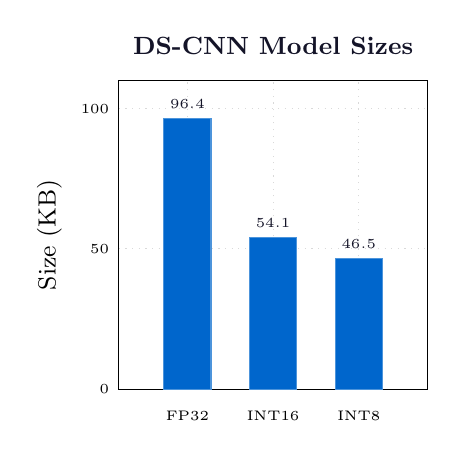
\begin{tikzpicture}
      \begin{axis}[
        ybar,
        width=5.5cm, height=5.5cm,
        bar width=0.6cm,
        symbolic x coords={FP32,INT16,INT8},
        xtick=data,
        ylabel={Size (KB)},
        ylabel style={font=\small},
        ymin=0, ymax=110,
        grid=major, grid style={dotted,gray!30},
        tick style={draw=none},
        ticklabel style={font=\tiny},
        title={DS-CNN Model Sizes},
        title style={font=\small\bfseries,color=ADIDark},
        nodes near coords,
        nodes near coords style={font=\tiny,color=ADIDark},
        enlarge x limits=0.4,
      ]
        \addplot[fill=ADIBlue,draw=ADIBlue!70] coordinates {
          (FP32,96.4)
          (INT16,54.1)
          (INT8,46.5)
        };
      \end{axis}
    \end{tikzpicture}
  \end{columns}

  \vspace{0.2cm}
  \begin{block}{TFLite Micro Deployment on MAX32690}
    {\small
    \begin{enumerate}
      \item Choose precision: \texttt{int8} for tightest fit in 3\,MB flash
      \item Compile with MSDK TFLite Micro library
      \item Load model binary, allocate tensor arena, invoke
    \end{enumerate}}
  \end{block}
\end{frame}

% ── PREPROCESSING 1: Vision ──────────────────────────────────
\begin{frame}{Preprocessing Pipeline — Vision}
  \renewcommand{\arraystretch}{1.3}
  \begin{tabular}{@{}>{\bfseries\small}l >{\small}c >{\small}l >{\small}l@{}}
    \toprule
    Model & Input Size & Resize Method & Normalization \\
    \midrule
    \rowcolor{ADIBlue!8}
    EfficientNetV2 & 112$\times$112 & Bilinear & $[-128, 127]$ INT8 scale \\
    MobileNetV2 & 32$\times$32 & Nearest & INT8 scale \\
    \rowcolor{ADIBlue!8}
    SimpleNet & 32$\times$32 & Nearest & INT8 scale \\
    U-Net & 48$\times$48 & Bilinear + fold(8) & INT8, 3ch → 48ch folded \\
    \rowcolor{ADIBlue!8}
    FPN & 256$\times$320 & Bilinear & INT8 scale \\
    TinierSSD & 120$\times$160 & Bilinear & INT8 scale \\
    \rowcolor{ADIBlue!8}
    VWW2 & 50$\times$50 & Bilinear & Greyscale + INT8 \\
    \bottomrule
  \end{tabular}

  \vspace{0.4cm}
  \begin{columns}[T]
    \column{0.48\textwidth}
    \begin{block}{AI8X Normalize}
      {\small\ttfamily
      class normalize:\\
      \quad def \_\_call\_\_(self, img):\\
      \quad\quad return img.sub(0.5).mul(256.)\\
      \quad\quad\quad\quad .round().clamp(-128,127)}
    \end{block}

    \column{0.48\textwidth}
    \begin{alertblock}{Channel Folding (U-Net)}
      {\small 3-channel 48×48 image → fold(8) → 3·64=192 channels at 6×6 spatial. Enables U-Net to fit within MAX78002 CNN layer limits.}
    \end{alertblock}
  \end{columns}
\end{frame}

% ── PREPROCESSING 2: Audio + Sensor ─────────────────────────
\begin{frame}{Preprocessing Pipeline — Audio \& Sensor}
  \begin{columns}[T]
    \column{0.48\textwidth}
    \begin{block}{Audio Preprocessing}
      \renewcommand{\arraystretch}{1.25}
      \begin{tabular}{@{}>{\bfseries\scriptsize}l >{\scriptsize}l@{}}
        \toprule
        Model & Pipeline \\
        \midrule
        DTLN & 16\,kHz → STFT (32\,ms) → magnitude (257) \\
             & + states (4 tensors) → 2-stage LSTMs \\[2pt]
        RNNoise & 16\,kHz → 10\,ms frames → 42 Bark features \\
                & INT8 normalize → GRU stack \\[2pt]
        GenreNet & GTZAN 22\,kHz → Mel-spectrogram 128$\times$128 \\
                 & FP32 → PyTorch Conv2D \\[2pt]
        DS-CNN & 16\,kHz → 40 MFCC + delta → 1$\times$490 \\[2pt]
        Conv1D & 16\,kHz → 128$\times$128 log-spectrogram \\
        \bottomrule
      \end{tabular}
    \end{block}

    \column{0.48\textwidth}
    \begin{block}{Sensor Preprocessing}
      \renewcommand{\arraystretch}{1.25}
      \begin{tabular}{@{}>{\bfseries\scriptsize}l >{\scriptsize}l@{}}
        \toprule
        Model & Pipeline \\
        \midrule
        Motor AE & ADC → 256-sample window × 3 axes \\
                 & → INT8 scale → Autoencoder \\[2pt]
        MIMII AE & Mic audio → 64-frame log-mel \\
                 & → 196$\times$640 spectrogram \\[2pt]
        MicroNet AD & Mic audio → 32-frame log-mel \\
                    & → 32$\times$32$\times$1 (greyscale) → INT8 \\
        \bottomrule
      \end{tabular}
    \end{block}
  \end{columns}

  \vspace{0.3cm}
  \begin{alertblock}{Key Principle}
    {\small Audio and sensor signals are transformed to \textbf{2D image-like tensors} (spectrograms, FFT frames), enabling standard 2D CNN operations on ADI's MAX78002 CNN accelerator.}
  \end{alertblock}
\end{frame}

% ── TOOLCHAIN 1: Ecosystem Table ────────────────────────────
\begin{frame}{Toolchain Ecosystem}
  \renewcommand{\arraystretch}{1.35}
  \begin{tabular}{@{}>{\bfseries\small\color{ADIBlue}}l >{\small}l >{\small}l@{}}
    \toprule
    Tool & Purpose & Source \\
    \midrule
    \rowcolor{ADIBlue!8}
    ai8xize.py & Synthesize AI8X model → MAX78002 HW config & MaximIntegratedAI/ai8x-synthesis \\
    ai8x-training & QAT training framework for MAX78000/78002 & MaximIntegratedAI/ai8x-training \\
    \rowcolor{ADIBlue!8}
    TFLite Micro & INT8 inference on MAX32690 (Cortex-M4F) & tensorflow/tflite-micro \\
    MSDK & Full SDK: BSP, drivers, peripheral examples & analogdevicesinc/msdk \\
    \rowcolor{ADIBlue!8}
    EV-Kit demos & Ready-to-flash firmware for eval kits & analogdevicesinc/msdk/Examples \\
    third\_party/ai8x & PyTorch shim: normalize, fold, inference & This repo \\
    \bottomrule
  \end{tabular}

  \vspace{0.5cm}
  \begin{columns}[T]
    \column{0.48\textwidth}
    \begin{block}{third\_party/ai8x/ Contents}
      {\small
      \begin{itemize}
        \item \texttt{ai8x.py} — normalize, fold/unfold, INT8 layers
        \item \texttt{ai8x\_blocks.py} — ResNet blocks, FPN building blocks
        \item \texttt{devices.py} — hardware limits (74 layers, 1024 ch)
        \item \texttt{util\_ai8x\_inference.py} — \texttt{AI8XInference} runner
      \end{itemize}}
    \end{block}

    \column{0.48\textwidth}
    \begin{alertblock}{AI8XInference API}
      \begin{lstlisting}[language=Python,basicstyle=\ttfamily\tiny]
from third_party.ai8x.util_ai8x_inference \
    import AI8XInference

model = AI8XInference(
    "data/model/ai87-fpn-qat8-q.pth.tar")
output = model.run(input_tensor)
      \end{lstlisting}
    \end{alertblock}
  \end{columns}
\end{frame}

% ── TOOLCHAIN 2: Dev Flow Diagram ────────────────────────────
\begin{frame}{Full Development Flow}
  \begin{center}
  \begin{tikzpicture}[
    node distance=0.5cm and 1.2cm,
    box/.style={draw=ADIBlue,fill=ADIBlue!10,rounded corners=5pt,
                font=\small\bfseries,inner sep=7pt,
                minimum width=2.4cm,minimum height=0.85cm,
                text=ADIDark,align=center,drop shadow},
    gbox/.style={box,fill=ADITeal!15,draw=ADITeal!70!black},
    rbox/.style={box,fill=ADIAmber!20,draw=ADIAmber!70!black},
    arr/.style={-{Stealth[scale=0.9]},very thick,color=ADIBlue},
    note/.style={font=\scriptsize\itshape,color=ADIGray,align=center}
  ]
    \node[box] (D) {Collect\\Data};
    \node[box,right=of D] (T) {Define Model\\(\texttt{ai8x} layers)};
    \node[gbox,right=of T] (Q) {QAT\\Training};
    \node[box,right=of Q] (S) {Synthesize\\(\texttt{ai8xize.py})};
    \node[rbox,right=of S] (F) {Flash to\\EV-Kit};
    \node[gbox,below=0.7cm of F] (E) {Evaluate\\Accuracy};
    \node[box,left=of E] (M) {Monitor\\Deployment};
    \node[box,left=of M] (P) {Package \&\\Version};
    \node[box,left=of P] (R) {CI\\Tests};

    \draw[arr] (D)--(T);
    \draw[arr] (T)--(Q);
    \draw[arr] (Q)--(S);
    \draw[arr] (S)--(F);
    \draw[arr] (F)--(E);
    \draw[arr] (E)--(M);
    \draw[arr] (M)--(P);
    \draw[arr] (P)--(R);
    \draw[arr] (R.west) -- ++(-0.4,0) |- ($(Q.south)+(0,-0.3)$) -- (Q.south)
      node[note,midway,below=2pt]{retrain if gate fails};

    \node[note,below=0.15cm of D] {MIMII, VOC,\\Speech Cmds};
    \node[note,above=0.15cm of Q] {ai8x-training};
    \node[note,above=0.15cm of S] {HW config};
    \node[note,above=0.15cm of F] {MSDK};
    \node[note,below=0.15cm of E] {edgeai-benchmark};
    \node[note,below=0.15cm of M] {MSE / PESQ drift};
    \node[note,below=0.15cm of R] {pytest CI};
  \end{tikzpicture}
  \end{center}
\end{frame}

% ── MLOPS 1: Pipeline Overview ──────────────────────────────
\begin{frame}{MLOps Pipeline — Overview}
  \begin{columns}[T]
    \column{0.52\textwidth}
    \begin{tikzpicture}[
      stage/.style={draw=ADIBlue,fill=ADIBlue!10,rounded corners=4pt,
                    font=\scriptsize\bfseries,inner sep=5pt,
                    minimum width=2.0cm,minimum height=0.7cm,
                    align=center},
      gstage/.style={stage,fill=ADITeal!15,draw=ADITeal},
      arr/.style={-{Stealth[scale=0.7]},ADIBlue,thick},
      lbl/.style={font=\tiny\itshape,color=ADIGray}
    ]
      \node[stage] (A) at (0,0) {1. Data\\Preparation};
      \node[stage] (B) at (0,-1.1) {2. QAT\\Training};
      \node[gstage] (C) at (0,-2.2) {3. Synthesize\\/ Export};
      \node[stage] (D) at (0,-3.3) {4. Evaluate\\(Accuracy)};
      \node[gstage] (E) at (0,-4.4) {5. Flash\\+ Monitor};
      \draw[arr] (A)--(B); \draw[arr] (B)--(C);
      \draw[arr] (C)--(D); \draw[arr] (D)--(E);
      \draw[arr,dashed,color=ADIRed] (D.east) -- ++(0.5,0) node[right,font=\tiny,color=ADIRed]{gate fail}
        |- ($(B.east)+(0.5,0)$) -- (B.east);
      \node[lbl,right=0.1cm of A] {MIMII, VOC, Speech V2};
      \node[lbl,right=0.1cm of B] {ai8x-training};
      \node[lbl,right=0.1cm of C] {ai8xize.py};
      \node[lbl,right=0.1cm of D] {pytest + benchmark};
      \node[lbl,right=0.1cm of E] {EV-Kit + drift detect};
    \end{tikzpicture}

    \column{0.45\textwidth}
    \begin{block}{Pipeline Components}
      {\small
      \begin{itemize}
        \item \textbf{model\_manager.py} — registry CRUD, artifact download
        \item \textbf{data\_pipeline.py} — domain-aware preprocessing (vision/audio/sensor)
        \item \textbf{evaluator.py} — accuracy gates with \texttt{AccuracyGateError}
        \item \textbf{artifact\_manager.py} — pack/unpack/verify bundles
        \item \textbf{monitor.py} — rolling latency, drift detection
        \item \textbf{train\_pipeline.py} — QAT → synthesize → evaluate
        \item \textbf{eval\_pipeline.py} — FP32 vs INT8 comparison
        \item \textbf{deploy\_pipeline.py} — bundle + flash/SCP push
      \end{itemize}}
    \end{block}
    \vspace{4pt}
    \begin{alertblock}{CI/CD}
      {\small 6-job GitHub Actions: lint → unit tests → eval matrix (vision/audio/sensor) → package → nightly}
    \end{alertblock}
  \end{columns}
\end{frame}

% ── MLOPS 2: Model Registry ─────────────────────────────────
\begin{frame}{MLOps Pipeline — Model Registry}
  \begin{columns}[T]
    \column{0.52\textwidth}
    \begin{block}{\texttt{model\_index.json} Structure}
      \begin{lstlisting}[language=json,basicstyle=\ttfamily\tiny]
{
  "uniqueId": "<uuid>",
  "name": "DS CNN",
  "task": "Keyword Spotting",
  "taskType": "Audio",
  "framework": "tensorflow",
  "license": "Apache-2.0",
  "owner": "ADI",
  "supportedPlatforms": [{
    "soc": "MAX32690",
    "board": "EvKit_V1",
    "family": "Cortex-M",
    "modelPaths": {
      "int8":    "path/to/model_int8.tflite",
      "float32": "path/to/model_float32.tflite"
    },
    "sizeInKb": {"int8": 46.5, "float32": 96.4},
    "compilation": {
      "optimization": {
        "values": ["-O0", "-O2"],
        "default": "-O0"
      },
      "quantization": {
        "values": ["int8","float32"],
        "default": "int8"
      }
    }
  }]
}
      \end{lstlisting}
    \end{block}

    \column{0.45\textwidth}
    \begin{block}{\texttt{ModelManager} Python API}
      \begin{lstlisting}[language=Python,basicstyle=\ttfamily\tiny]
from mlops.model_manager import ModelManager

mgr = ModelManager("config/pipeline.yaml")

# List models by domain
vision = mgr.list_models(domain="Vision")
audio  = mgr.list_models(domain="Audio")

# Get artifact path
path = mgr.get_artifact(
    "DS CNN", soc="MAX32690",
    precision="int8")

# Get accuracy
acc = mgr.get_accuracy(
    "DS CNN", precision="int8")
# -> {"accuracy": 0.9452, "size_kb": 46.5}

# Register new model
mgr.register("MyModel", {
    "task": "Keyword Spotting",
    "format": "tflite",
    "platforms": ["MAX32690"]
})
      \end{lstlisting}
    \end{block}
    \vspace{4pt}
    \begin{alertblock}{Schema Validation}
      {\small \texttt{models.schema.json} validates every entry in \texttt{model\_index.json}. New models auto-checked on PR.}
    \end{alertblock}
  \end{columns}
\end{frame}

% ── MLOPS 3: Evaluation & CI ────────────────────────────────
\begin{frame}{MLOps Pipeline — Evaluation \& CI/CD}
  \begin{columns}[T]
    \column{0.5\textwidth}
    \begin{block}{Accuracy Gates}
      \renewcommand{\arraystretch}{1.25}
      \begin{tabular}{@{}>{\small\bfseries}l >{\small}l >{\small}r@{}}
        \toprule
        Domain & Metric & Max Drop \\
        \midrule
        Vision-Cls & Top-1 Acc & 2.0 pp \\
        Vision-Det & mAP & 1.0 pp \\
        Vision-Seg & pixel Acc & 1.5 pp \\
        Audio-KWS & Accuracy & 1.5 pp \\
        Audio-PESQ & PESQ score & 0.05 \\
        Sensor-MSE & Recon MSE & 10\% rel \\
        \bottomrule
      \end{tabular}
      \vspace{4pt}
      {\small Gate fail → \texttt{AccuracyGateError} → CI fail → trigger QAT retrain job}
    \end{block}

    \column{0.47\textwidth}
    \begin{block}{GitHub Actions CI (\texttt{mlops\_ci.yml})}
      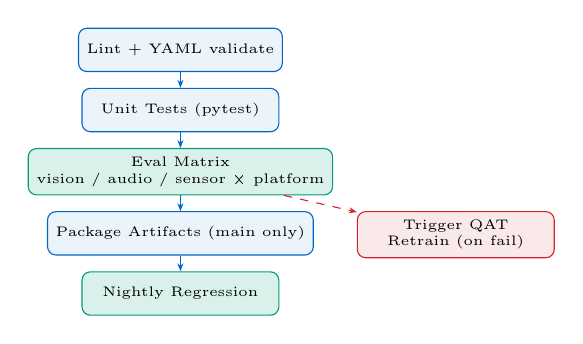
\begin{tikzpicture}[
        job/.style={draw=ADIBlue,fill=ADIBlue!8,rounded corners=3pt,
                    font=\tiny,inner sep=3pt,minimum width=2.5cm,
                    minimum height=0.55cm,align=center},
        gjob/.style={job,fill=ADITeal!15,draw=ADITeal},
        rjob/.style={job,fill=ADIRed!10,draw=ADIRed},
        arr/.style={-{Stealth[scale=0.6]},ADIBlue}
      ]
        \node[job] (L) {Lint + YAML validate};
        \node[job,below=0.2cm of L] (U) {Unit Tests (pytest)};
        \node[gjob,below=0.2cm of U] (E) {Eval Matrix\\vision / audio / sensor × platform};
        \node[job,below=0.2cm of E] (P) {Package Artifacts (main only)};
        \node[rjob,right=0.3cm of E,yshift=-0.8cm] (R) {Trigger QAT\\Retrain (on fail)};
        \node[gjob,below=0.2cm of P] (N) {Nightly Regression};
        \draw[arr] (L)--(U); \draw[arr] (U)--(E);
        \draw[arr] (E)--(P); \draw[arr] (P)--(N);
        \draw[arr,dashed,color=ADIRed] (E)--(R);
      \end{tikzpicture}
    \end{block}
    \vspace{4pt}
    \begin{alertblock}{Eval Matrix}
      {\small \textbf{3 domains} × \textbf{3 platforms} = 9 parallel evaluation jobs per push}
    \end{alertblock}
  \end{columns}
\end{frame}

% ── MLOPS 4: Code Structure ──────────────────────────────────
\begin{frame}{MLOps Code Structure}
  \begin{columns}[T]
    \column{0.48\textwidth}
    \begin{block}{Directory Layout (\texttt{code-adi/})}
      \begin{tikzpicture}[
        dir/.style={font=\scriptsize\ttfamily\bfseries\color{ADIBlue}},
        fil/.style={font=\scriptsize\ttfamily\color{ADIDark}},
        every node/.style={anchor=west}
      ]
        \node[dir] at (0,0) {\faFolder\ code-adi/};
        \node[dir] at (0.3,-0.35) {\faFolder\ config/};
        \node[fil] at (0.6,-0.65) {pipeline\_config.yaml};
        \node[fil] at (0.6,-0.95) {model\_registry.yaml};
        \node[dir] at (0.3,-1.3) {\faFolder\ mlops/};
        \node[fil] at (0.6,-1.6) {model\_manager.py};
        \node[fil] at (0.6,-1.9) {data\_pipeline.py};
        \node[fil] at (0.6,-2.2) {evaluator.py};
        \node[fil] at (0.6,-2.5) {artifact\_manager.py};
        \node[fil] at (0.6,-2.8) {monitor.py};
        \node[dir] at (0.3,-3.15) {\faFolder\ pipelines/};
        \node[fil] at (0.6,-3.45) {train\_pipeline.py};
        \node[fil] at (0.6,-3.75) {eval\_pipeline.py};
        \node[fil] at (0.6,-4.05) {deploy\_pipeline.py};
        \node[dir] at (0.3,-4.4) {\faFolder\ tests/};
        \node[fil] at (0.6,-4.7) {test\_pipeline.py};
      \end{tikzpicture}
    \end{block}

    \column{0.48\textwidth}
    \begin{block}{Module Responsibilities}
      \renewcommand{\arraystretch}{1.2}
      {\small
      \begin{tabular}{@{}>{\ttfamily\scriptsize}l >{\scriptsize}l@{}}
        \toprule
        Module & Responsibility \\
        \midrule
        model\_manager & Registry CRUD, artifact paths \\
        data\_pipeline & Domain preprocessing\\
                       & (vision/audio/sensor) \\
        evaluator & Accuracy metrics + gates \\
        artifact\_manager & Bundle pack/unpack/verify \\
        monitor & Latency, drift, alerts \\
        train\_pipeline & QAT → synthesize → eval \\
        eval\_pipeline & FP32 vs INT8 comparison \\
        deploy\_pipeline & Bundle + flash/SCP push \\
        \bottomrule
      \end{tabular}}
    \end{block}
    \vspace{4pt}
    \begin{alertblock}{Quick Start}
      {\small\ttfamily
      \$ cd code-adi\\
      \$ python pipelines/eval\_pipeline.py\\
      \quad --model "DS CNN" --soc MAX32690}
    \end{alertblock}
  \end{columns}
\end{frame}

% ── COMPARISON: ADI vs TI ────────────────────────────────────
\begin{frame}{ADI Model Zoo vs.\ TI EdgeAI Model Zoo}
  \begin{columns}[T]
    \column{0.05\textwidth}
    \column{0.44\textwidth}
    \begin{block}{\textcolor{ADIBlue}{\faChartBar\ ADI Model Zoo}}
      {\small
      \begin{itemize}
        \item \alert{$\sim$15} models
        \item Domains: Vision, \textbf{Audio}, \textbf{Sensor}
        \item Target: MCU/DSP — \alert{$\mu$W–mW} range
        \item Format: AI8X (proprietary), TFLite, PyTorch
        \item HW: MAX78002, MAX32690, ADSP-SC835
        \item Use case: \textbf{TinyML, IoT, wearables}
        \item Models stored \textbf{directly in repo}
        \item Inference: AI8X CNN accelerator, TFLite Micro
        \item Dataset: CIFAR-100, VOC, Speech Cmds, MIMII
      \end{itemize}}
    \end{block}
    \column{0.44\textwidth}
    \begin{block}{\textcolor{ADIGray}{\faChartBar\ TI EdgeAI Model Zoo}}
      {\small
      \begin{itemize}
        \item \alert{180+} models
        \item Domain: Vision \textbf{only}
        \item Target: SoC/MPU — \alert{W} range
        \item Format: ONNX, TFLite, TVM-compiled
        \item HW: TDA4VM, AM62A–AM69A
        \item Use case: \textbf{ADAS, robotics, cameras}
        \item Models via \textbf{.link} file download
        \item Inference: TIDL, onnxrt, tflitert, tvmrt
        \item Dataset: ImageNet, COCO, Cityscapes
      \end{itemize}}
    \end{block}
    \column{0.07\textwidth}
  \end{columns}

  \vspace{0.4cm}
  \renewcommand{\arraystretch}{1.2}
  \begin{tabular}{@{}>{\bfseries\small}l >{\small\color{ADIBlue}}c >{\small}c@{}}
    \toprule
    Dimension & ADI & TI \\
    \midrule
    Model count & $\sim$15 & 180+ \\
    Power budget & $<$6\,mW & 1–32\,TOPS \\
    INT8 method & QAT (AI8X) & QAT / PTQ \\
    Multi-domain & \textcolor{ADITeal}{\checkmark} & \textcolor{ADIRed}{$\times$} \\
    Ultra-low-power & \textcolor{ADITeal}{\checkmark} & \textcolor{ADIRed}{$\times$} \\
    \bottomrule
  \end{tabular}
\end{frame}

% ── SUMMARY 1: Key Strengths ────────────────────────────────
\begin{frame}{Summary — Key Strengths}
  \begin{columns}[T]
    \column{0.48\textwidth}
    \begin{block}{\adi{Multi-Domain Coverage}}
      {\small Vision + Audio + Sensor in one repo — unique among edge AI model zoos. Deploy the same pipeline across camera, microphone, and vibration sensor nodes.}
    \end{block}
    \vspace{4pt}
    \begin{block}{\adi{Self-Contained Models}}
      {\small Every model includes sample data, preprocessing, inference script, and requirements. Clone → install → run in $<$5 minutes.}
    \end{block}
    \vspace{4pt}
    \begin{block}{\adi{QAT First-Class}}
      {\small AI8X format is designed from the ground up for INT8 QAT. No accuracy surprise at deployment — the model was trained as INT8.}
    \end{block}

    \column{0.48\textwidth}
    \begin{block}{\adi{Ultra-Low-Power Targets}}
      {\small MAX78002 CNN accelerator at $<$6\,mW enables always-on computer vision and audio classification on coin-cell batteries.}
    \end{block}
    \vspace{4pt}
    \begin{block}{\adi{Schema-Validated Registry}}
      {\small \texttt{model\_index.json} + \texttt{models.schema.json} ensures consistent metadata, per-platform paths, and compilation options for every model.}
    \end{block}
    \vspace{4pt}
    \begin{alertblock}{15+ Models, 3 Domains, 3 Platforms}
      {\small The ADI Model Zoo covers the full spectrum of embedded edge AI — from image classification to motor fault detection — all on Analog Devices silicon.}
    \end{alertblock}
  \end{columns}
\end{frame}

% ── SUMMARY 2: Next Steps ───────────────────────────────────
\begin{frame}{Next Steps \& Resources}
  \begin{columns}[T]
    \column{0.48\textwidth}
    \begin{block}{Getting Started}
      {\small
      \begin{enumerate}
        \item Clone the repo:\\
              {\ttfamily git clone https://github.com/analogdevicesinc/adi-model-zoo}
        \item Pick a model and install deps:\\
              {\ttfamily cd vision\_models/object\_detection/feature\_pyramid\_net}\\
              {\ttfamily pip install -r requirements.txt}
        \item Run inference:\\
              {\ttfamily python example.py data/input/input.jpg}
        \item Explore \texttt{model\_index.json} for your target SoC
        \item Train / fine-tune with \texttt{ai8x-training}
        \item Synthesize with \texttt{ai8xize.py} → flash EV-Kit
      \end{enumerate}}
    \end{block}

    \column{0.48\textwidth}
    \begin{block}{Key Resources}
      {\small
      \begin{itemize}
        \item \textbf{ADI Model Zoo}:\\
              {\ttfamily\scriptsize github.com/analogdevicesinc/adi-model-zoo}
        \item \textbf{MSDK (MAX SDK)}:\\
              {\ttfamily\scriptsize github.com/analogdevicesinc/msdk}
        \item \textbf{ai8x-training}:\\
              {\ttfamily\scriptsize github.com/MaximIntegratedAI/ai8x-training}
        \item \textbf{ai8x-synthesis}:\\
              {\ttfamily\scriptsize github.com/MaximIntegratedAI/ai8x-synthesis}
        \item \textbf{TFLite Micro}:\\
              {\ttfamily\scriptsize github.com/tensorflow/tflite-micro}
        \item \textbf{MIMII Dataset}:\\
              {\ttfamily\scriptsize zenodo.org/record/3384388}
      \end{itemize}}
    \end{block}
  \end{columns}

  \vspace{0.3cm}
  \begin{center}
    
\begin{tikzpicture}
      \fill[ADIBlue] (0,0) rectangle (0.45\textwidth,4pt);
      \fill[ADITeal] (0.47\textwidth,0) rectangle (0.94\textwidth,4pt);
    \end{tikzpicture}\\[4pt]
    {\small\color{ADIGray} Analog Devices, Inc.\ — Intelligent Edge AI}
  \end{center}
\end{frame}

\end{document}
